\documentclass{beamer}
%\documentclass[handout]{beamer} %use this for no pauses
\usepackage{fancyvrb}
\usepackage{color}
\definecolor{forestgreen(web)}{rgb}{0.13, 0.55, 0.13}
\definecolor{cardinal}{rgb}{0.77, 0.12, 0.23}
\mode<presentation>
{
  \definecolor{berkeleyblue}{HTML}{003262}
  \definecolor{berkeleygold}{HTML}{FDB515}
  \usetheme{Boadilla}      % or try Darmstadt, Madrid, Warsaw, Boadilla...
  %\usecolortheme{dove} % or try albatross, beaver, crane, ...
  \setbeamercolor{structure}{fg=berkeleyblue,bg=berkeleygold}
  \setbeamercolor{palette primary}{fg=berkeleyblue,bg=berkeleygold} % changed this
  \setbeamercolor{palette secondary}{bg=berkeleyblue,fg=white} % changed this
  \setbeamercolor{palette tertiary}{bg=berkeleyblue,fg=white} % changed this
  \usefonttheme{structurebold}  % or try serif, structurebold, ...
  \useinnertheme{circles}
  \setbeamertemplate{navigation symbols}{}
  \setbeamertemplate{caption}[numbered]
  \usebackgroundtemplate{}
}

% adding slide numbers
\addtobeamertemplate{navigation symbols}{}{%
    \usebeamerfont{footline}%
    \usebeamercolor[fg]{footline}%
    \hspace{1em}%
    \insertframenumber/\inserttotalframenumber
}

\renewcommand{\(}{\begin{columns}}
\renewcommand{\)}{\end{columns}}
\newcommand{\<}[1]{\begin{column}{#1}}
\renewcommand{\>}{\end{column}}

% equation stuff
\newcommand{\Macro}{\ensuremath{\Sigma}}
\newcommand{\Sn}{\ensuremath{S_N} }
\newcommand{\vOmega}{\ensuremath{\hat{\Omega}}}
\usepackage{mathrsfs}
\usepackage[mathcal]{euscript}
\usepackage{amssymb}
\usepackage{amsthm}
\usepackage{epsfig}
\usepackage{amsmath}

\newcommand{\ve}[1]{\ensuremath{\mathbf{#1}}}
\newcommand{\micro}{\ensuremath{\sigma}}
\newcommand{\detR}{\ensuremath{\Sigma}}

\title{PyNE Software Library: an Overview}
\author{R.\ N.\ Slaybaugh}
\date{22 October 2014}
%%%%%%%%%%%%%%%%%%%%%%%%%%%%%%%%%%%%%%%%%%%%%%%%%%%%%%
\begin{document}

%%%%%%%%%%%%%%%%%%%%%%%%%%%%%%%%%%%%%%%%%%%%%%%%%%%%%%
%%%%%%%%%%%%%%%%%%%%%%%%%%%%%%%%%%%%%%%%%%%%%%%%%%%%%%
\begin{frame}
\title{PyNE Software Library: an Overview}
\subtitle{ANS Nor Cal Meeting}
\author{
        \includegraphics[height=2cm]{../bk}\\R.\ N.\ Slaybaugh, \\ Univ. of Cal.\ Berkeley}

\date{22 October 2014\\ Alfred's Stakehouse, San Francisco}
\titlepage
\end{frame}


\begin{frame}{Outline}
	\begin{itemize}
    \item
	\end{itemize}
\end{frame}

\begin{frame}{WARP \cite{pyne}}
	\begin{itemize}
	\item
	\end{itemize}
\end{frame}

\begin{frame}{Software Verification and Validation}
	\begin{itemize}
	\pause
	\item{Ensuring that software meets its specifications and fulfills its intended purpose}
	\pause
	\item{Validation: ``Are we building the right thing?"}
	\pause
	\item{Verification: ``Are we building the thing right?"}
	\pause
	\item{Test cases are an important part of software V\&V}
	\end{itemize}
\end{frame}



% --------------------------------------------------------------
\section*{}
\begin{frame}[fragile]
  \frametitle{Questions?}
  \begin{center}
  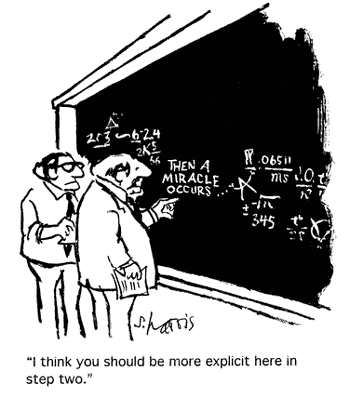
\includegraphics[height=3in,clip]{../questions-comic}  
  \end{center}
  
\end{frame}

\begin{frame}[plain,noframenumbering]{References}
	\bibliographystyle{unsrt}
	\bibliography{2014-10-norcal-ans-pyne.bib}
\end{frame}

\end{document}
